\documentclass[11pt,twoside,openright,a4paper]{report}

\usepackage{tocloft}
%\usepackage{graphicx}
\usepackage{amsmath,amsfonts}
\usepackage{amssymb}
%\usepackage{math}
\usepackage[utf8]{inputenc}
\usepackage[francais]{babel}

\usepackage{tikz}
\usetikzlibrary{mindmap}
\pagestyle{empty}


\selectlanguage{francais}

\oddsidemargin 0.8cm
\evensidemargin -0.2cm
\textwidth 15cm
\textheight 23cm
\topmargin -0.5cm

\renewcommand{\familydefault}{\sfdefault}

% table of contents config

\tocloftpagestyle{empty}
\setcounter{tocdepth}{1}

%

%\usepackage{sectsty}
\usepackage{fancyhdr}

\renewcommand{\chaptermark}[1]{\markboth{\thechapter\quad #1}{}}
\renewcommand{\sectionmark}[1]{\markright{#1\quad \thesection}}
\lhead[\fancyplain{}{\raggedright\slshape\leftmark}]{}
\chead{}
\rhead[]{\fancyplain{}{\raggedleft\slshape\rightmark}}
\lfoot[\fancyplain{}{\thepage}]{}
\cfoot{}
\rfoot[]{\fancyplain{\thepage}{\thepage}}

%\setlength{\headrulewidth}{0.4pt}
%\setlength{\footrulewidth}{0.4pt}
%\setlength{\plainfootrulewidth}{0.4pt}

\usepackage{listings}
\usepackage{xcolor}

\begin{document}

\begin{titlepage}
\begin{Large}
\baselineskip=7mm
\noindent
\hfill

\begin{center}
\rule{\textwidth}{0.5 mm}\\
{\huge\sffamily\bfseries\baselineskip=1cm
Cours de théorie des langages
\par}
\rule{\textwidth}{0.5 mm}\\
{\Large\sffamily\bfseries Licence 3}
\vskip 5mm
23/06/2014
\end{center}

\vfill

\end{Large}
\end{titlepage}

\cleardoublepage

\tableofcontents

\pagestyle{fancy}

% \chapter{Introduction} % (fold)
\label{cha:introduction}


\section{Historique} % (fold)
\label{sec:historique}

Chomsky est un linguiste américain voulant formaliser le langage naturel. Grâce aux grammaires génératrices et transformationnelles, en 1950, il est à réussi à créer la hiérarchie de Chomsky, permettant de classer les langages.

En 1960, Schützenber et Mivat ont développé les langages informatiques grâce aux travaux de Chomsky.

% section historique (end)


\section{Utilité} % (fold)
\label{sec:utilit_}

L'utilisation des travaux de Chomsky pour les langages informatiques servent comme :
\begin{itemize}
	\item D'Outil théorique, permettant d'écrire des règles d'un langage, grâce aux grammaires.
	\item L'analyse syntaxe, permettant de reconnaître, si un texte respecte la syntaxe d'un langage.
	\item L'analyse sémantique, donnant un sens à un texte syntaxiquement correct.
	\item La compilation, traduisant le texte d'un langage dans un autre.
\end{itemize}

% section utilit_ (end)


% chapter introduction (end)

\chapter{Introduction} % (fold)
\label{cha:introduction}


\section{Historique} % (fold)
\label{sec:historique}

Chomsky est un linguiste américain voulant formaliser le langage naturel. Grâce aux grammaires génératrices et transformationnelles, en 1950, il est à réussi à créer la hiérarchie de Chomsky, permettant de classer les langages.

En 1960, Schützenber et Mivat ont développé les langages informatiques grâce aux travaux de Chomsky.

% section historique (end)


\section{Utilité} % (fold)
\label{sec:utilit_}

L'utilisation des travaux de Chomsky pour les langages informatiques servent comme :
\begin{itemize}
	\item D'Outil théorique, permettant d'écrire des règles d'un langage, grâce aux grammaires.
	\item L'analyse syntaxe, permettant de reconnaître, si un texte respecte la syntaxe d'un langage.
	\item L'analyse sémantique, donnant un sens à un texte syntaxiquement correct.
	\item La compilation, traduisant le texte d'un langage dans un autre.
\end{itemize}

% section utilit_ (end)


% chapter introduction (end)

\chapter{Les généralités sur les langages} % (fold)
\label{cha:les_g_n_ralit_s_sur_les_langages}


\section{Alphabet et mot} % (fold)
\label{sec:alphabet_et_mot}


\paragraph{Définition} % (fold)
\label{par:d_finition}

Un alphabet est un ensemble fini de symboles appelés aussi lettres ou caractères. Les alphabets sont notés $\Sigma$ et les lettres les composant sont notées en minuscules.

% paragraph d_finition (end)


\paragraph{Exemples} % (fold)
\label{par:exemples}


\begin{itemize}
	\item $\Sigma_1 = \{a,b,c,d,e,f,g,\ldots,z\}$
	\item $\Sigma_2 = \{0,1,\ldots,9\}$
	\item $\Sigma_3 = \{0,1\}$
	\item $\Sigma_4 = \{class\ ,\ public\ ,\ static\ ,\ void\ ,\ int\ ,\ \ldots\}$
\end{itemize}


% paragraph exemples (end)


\paragraph{Définition} % (fold)
\label{par:d_finition}

Un mot sur un alphabet $\Sigma$ est une suite finie de symbole de $\Sigma$.

% paragraph d_finition (end)


\paragraph{Définition} % (fold)
\label{par:d_finition}

La longueur d'un mot est le nombre de symboles que compose un mot. Soit un mot w la longueur d'un mot est noté $\left|w\right|$. D'une manière plus formel un mot w de longueur n sur l'alphabet $\Sigma$ est une application de \{1,2,...,n\} dans l'alphabet $\Sigma$ qui associe à chaque entier $i \in \{1,2,...,n\}$ le i\up{ème} symbole de w.

% paragraph d_finition (end)


\paragraph{Exemples} % (fold)
\label{par:exemples}

\begin{itemize}
	\item Soit l'alphabet $\Sigma=\{a,b,c\}$ et w l'application de \{1,2,3,4\} dans $\Sigma$ définie par w(1)=a, w(2)=c, w(3)=a, w(4)=b. w est un mot de longueur 4, noté $\left|w\right| = 4$.
	\item La suite vide de symbole de $\Sigma$ est une unique application de $\varnothing$ dans $\Sigma$. Elle est appelé le mot vide noté $\epsilon$. La longueur du mot vide est de 0, $\left|\epsilon\right| = 0$.
\end{itemize}


% paragraph exemples (end)


\paragraph{Définition} % (fold)
\label{par:d_finition}

L’occurrence d'une lettre dans un mot est l'apparition de cette lettres dans le mot. Pour un mot w donné, le nombre d'occurrence d'une lettre x dans w est noté $\left|w\right|_x=n$.

% paragraph d_finition (end)


\paragraph{Exemple} % (fold)
\label{par:exemple}

Soit l'alphabet $\Sigma=\{a,b,c\}$ et 2 mots $u=acab$ et $v=bb$.

\begin{itemize}
	\item La lettre $a$ a 2 occurrences dans le mot u. On peut donc noté $\left|u\right|_a=2$.
	\item $\left|u^3\right|_{ab}=3 ; \left|u^3\right|_u=3 ; \left|v^2\right|_v=3 $
\end{itemize}

% paragraph exemple (end)


\paragraph{Remarque} % (fold)
\label{par:remarque}

$\left|w\right|=\sum\limits_{x\in\Sigma} \left|w\right|_x$

% paragraph remarque (end)


\paragraph{Définition} % (fold)
\label{par:d_finition}

L'ensemble de tous mots est noté $\Sigma^*$. Si $\Sigma$ n'est pas vide alors $\Sigma^*$ est infini mais dénombrable.

% paragraph d_finition (end)


\paragraph{Remarques} % (fold)
\label{par:remarques}

\begin{itemize}
	\item Il ne faut pas confondre mot et symbole.
	\item $\epsilon \in \Sigma^*$ mais $\epsilon \not \in \Sigma$
\end{itemize}

% paragraph remarques (end)


% section alphabet_et_mot (end)


\section{Monoïde ($\Sigma^*,.$)} % (fold)
\label{sec:mono_de_}

\paragraph{Définition} % (fold)
\label{par:d_finition}

Un monoïde est composé d'une loi de composition interne associative et d'un élément neutre.

% paragraph d_finition (end)


\paragraph{Définition} % (fold)
\label{par:d_finition}

La concaténation est une opération binaire interne sur $\Sigma^*$,noté . , et défini par :
	
	\begin{itemize}
		\item $\forall(u,v)\in \Sigma^*, \left|u.v\right|=\left|u\right|+\left|v\right|$
		\item $\forall i\leq \left|u\right|,(u.v)(i)=u(i)$
		\item $\forall i\leq \left|v\right|,(u.v)(\left|u\right|+i)=v(i)$
	\end{itemize}

% paragraph d_finition (end)


\paragraph{Définition} % (fold)
\label{par:d_finition}

L'opération associative est défini par les règles suivantes :

	\begin{itemize}
		\item $\forall(u,v,w) \in \Sigma^*,(u.v).w=u.(v.w)$
		\item Un élément neutre $\epsilon, \forall u \in \Sigma^*, \epsilon.u=u.\epsilon=u$
	\end{itemize}

% paragraph d_finition (end)


\paragraph{Remarque} % (fold)
\label{par:remarque}

La concaténation est non commutative c'est-à-dire qu'en général $u.v \neq v.u$

% paragraph remarque (end)


La puissance n d'un mot w, noté $w^n$, est la concaténation de w n fois.

\paragraph{Définition} % (fold)
\label{par:d_finition}
Soit un mot w, on a :

\begin{itemize}
	\item $w^0 = \epsilon$
	\item $\forall i \in \mathbb{N} , w^{i+1}=w^i.w$
\end{itemize}

% paragraph d_finition (end)


\paragraph{Exemples} % (fold)
\label{par:exemples}

Soit l'alphabet $\Sigma = \{a,b,c\}$ et $u$ et $v$ 2 mots tel que $u=abac$ et $v=bb$, on peut avoir:
\begin{itemize}
	\item $u.v=abacbb$
	\item $u^3=abacabacabac$
	\item $v^0=\epsilon$
	\item $\epsilon^5=\epsilon$
\end{itemize}

% paragraph exemples (end)


\paragraph{Définition} % (fold)
\label{par:d_finition}

Un mot $v$ est un facteur de $w$, s'il existe 2 mots $u_1 \in \Sigma^*$ et $u_2 \in \Sigma^*$ tel que $w=u_1vu_2$. On peut avoir les cas suivants :

\begin{itemize}
	\item Si $u_1=\epsilon$, $v$ est un facteur gauche ou préfixe de $w$
	\item Si $u_2=\epsilon$, $v$ est un facteur droite ou suffixe de $w$
	\item Si $u_1=\epsilon$ et $u_2=\epsilon$, $v$ est un facteur propre de $w$
\end{itemize}

% paragraph d_finition (end)


% section mono_de_ (end)


\section{Langage} % (fold)
\label{sec:langage}


\paragraph{Définition} % (fold)
\label{par:d_finition}

Le langage sur un alphabet $\Sigma$ est un ensemble de mot sur $\Sigma$, qui peut être fini ou infini. On prend pour notation pour les langages des lettres majuscules.

% paragraph d_finition (end)


\paragraph{Exemples} % (fold)
\label{par:exemples}

Soit le l'alphabet $\Sigma=\{a,b,c\}$, on a :

\begin{itemize}
	\item $A=\{a,bb,abac,bba,aaa\}$, un langage contenant 5 mots.
	\item $B=\varnothing$, un langage contenant aucun mot.
	\item $C=\{\epsilon\}$, un langage contenant 1 mot.
	\item $D=\{w \in \Sigma^* \mid \left|w\right|_c=0\}$ est un langage ne contenant aucun symbole $c$.
\end{itemize}

% paragraph exemples (end)


\paragraph{Remarque} % (fold)
\label{par:remarque}

Le langage vide est représenté par le symbole $\varnothing$ qui est différent du mot vide représenté par $\epsilon$.

% paragraph remarque (end)


\paragraph{Définition} % (fold)
\label{par:d_finition}

Les langages sont des ensembles donc on peut utiliser toutes les opérations ensemblistes.

% paragraph d_finition (end)


\paragraph{Exemple} % (fold)
\label{par:exemple}

Soient 2 langages A et B, on peut avoir les langages suivants : $A \cap B$, $A \cup B$, $A \setminus B$, $\overline{A}$ (complémentaire du langage A par rapport à $\Sigma$).

% paragraph exemple (end)


\paragraph{Définition} % (fold)
\label{par:d_finition}

La concaténation s'étant aux langages, noté . , de la manière suivante. Soient A et B 2 langages dans l'alphabet $\Sigma^*$, on a $A.B=\{u.v \mid a \in A et v \in B\}$. La concaténation est distributive par rapport à l'Union mais pas par rapport à l'Instersection. 

% paragraph d_finition (end)


\paragraph{Remarques} % (fold)
\label{par:remarques}

\begin{itemize}
	\item $\varnothing.A=\varnothing$ mais $\{\epsilon\}.A=A$.
	\item $\mathcal{P}(\Sigma^*)$ est l'ensemble des parties de $\Sigma^*$.
	\item $(\mathcal{P}(\Sigma^*),.)$ est un monoïde.
\end{itemize}

% paragraph remarques (end)


\paragraph{Définition} % (fold)
\label{par:d_finition}

La puissance $n$ d'un langage noté $A^n$ est défini par :
\begin{itemize}
	\item $A^0=\{\epsilon\}$
	\item $\forall i \in \mathbb{N}, A^{i+i}=A^i.A$
\end{itemize}

% paragraph d_finition (end)


\paragraph{Définitions} % (fold)
\label{par:d_finitions}

L'Etoile, ou Itération, ou Fermeture ou clôture de Kleene, d'un langage $A$, noté $A^*$, défini par :

$A^* = \bigcup\limits_{i \in \mathbb{N}} A^i = A^0 \cup A^1 \cup ...$

L'étoile propre de $A$, noté $A^+$ défini par :

$A^+ = \bigcup\limits_{i\in \mathbb{N^*}} A^i = A^1 \cup A^2 \cup ...$

% paragraph d_finitions (end)


\paragraph{Remarques} % (fold)
\label{par:remarques}

$A^+ = A.A^*$

$A^* = A^0 \cup A^+$

Si $\epsilon \in A$ alors $w \in A^+$ et $A^+ = A^*$
$A^*$ est le plus petit langage qui contient $A$, $\{\epsilon\}$ et qui est stable, ou fermé, par concaténation.

Si l'on considère l'alphabet $\Sigma$ comme un langage, contenant tous les mots de longueur 1. Pour tout $i \in \mathbb{N}$, $\Sigma^i$ est le langage de longueur $i$, alors $\Sigma^*$ est le langage de tous les mots.

% paragraph remarques (end)


% section langage (end)


% chapter les_g_n_ralit_s_sur_les_langages (end)

\chapter{Grammaires} % (fold)
\label{cha:grammaires}


\section{Comment définir un langage} % (fold)
\label{sec:comment_d_finir_un_langage}

\begin{itemize}
	\item On peut définir un langage par une phrase en Français.
	
	\paragraph{Exemple} % (fold)
	\label{par:exemple}

	$\mathcal{L}_p$ est le langage de tous les mots de longueur pair sur un l'alphabet $\{a,b\}$\\

	% paragraph exemple (end)


	\item Si le langage est fini, on peut donner, énumérer tous ses éléments(Définition en extension).

	\paragraph{Exemple} % (fold)
	\label{par:exemple}

	$A=\{\epsilon, a, bb, abab\}$\\
	
	% paragraph exemple (end)


	\item Un langage peut être défini par une propriété caractéristique de ses mots(Définition en extension).

	\paragraph{Exemple} % (fold)
	\label{par:exemple}

	$\mathcal{L}_p = \{w \in \{a,b\}^* \mid \forall n \in \mathbb{N}, \left|w\right|=2*n\}$\\
	
	% paragraph exemple (end)


	\item Un langage peut être défini à partir d'un autre langage par des opérations ensemblistes tels que Union, Intersection, Différence, Complémentation, Étoile, ...\\


	\item Un langage peut se définir de manière opérationnelle en donnant un algorithme de décision (fonction booléenne), qui prend en entré un mot quelconque et indique si le mot fait parti ou non du langage. La notion d'automate donne un formalisme opérationnel pour décider de l'appartenance d'un mot à un langage (reconnaître, accepter un mot).

	\paragraph{Exemple} % (fold)
	\label{par:exemple}

	Est ce que un mot $w \in \mathcal(L)_p$. On peut écrire un algorithme qui compte le nombre de caractères du mot $w$ et vérifie si le résultat est paire ou on se contente d'un automate à 2 états qui compte le nombre de symbole modulo 2.\\
	
	% paragraph exemple (end)


	\item On peut donner un procéder de génération de l'ensemble des mots du langage. La notion de grammaire est un formalisme qui permet de générer, engendrer l'ensemble des mots d'un langage.\\

	\paragraph{Exemples} % (fold)
	\label{par:exemples}

	\begin{itemize}
		\item On peut définir indirectement le langage $\mathcal{L}_p$ avec les règles suivantes :\\
		$\epsilon \in \mathcal{L}_p$.\\
		Si un mot $w \in \mathcal{L}_p$, alors $aaw \in \mathcal{L}_p$, $baw \in \mathcal{L}_p$, $abw \in \mathcal{L}_p$ et $bbw \in \mathcal{L}_p$.

		\item Soit $\mathcal{A}$ un langage défini sur l'alphabet $\Sigma = \{a,b\}$, on peut avoir :\\
		$\epsilon \in \mathcal{A}$.\\
		Si le mot $w \in \mathcal{A}$ alors $awb \in \mathcal{A}$.
		$\mathcal{A} = \{w \in \{a,b\} \mid \exists \mathbb{N}, w=a^nb^n\}$
	\end{itemize}

	% paragraph exemples (end)


\end{itemize}

% section comment_d_finir_un_langage (end)


\section{Grammaire formelle} % (fold)
\label{sec:grammaire_formelle}

Une grammaire est un ensemble de règles qui permettent de produire, générer, engendre, les mots d'un langage.


\paragraph{Définition} % (fold)
\label{par:d_finition}

Une grammaire est un quadruplet $(\Sigma,N,P,S)$ où :

\begin{itemize}
	\item $\Sigma$ est un alphabet, un ensemble fini de symboles terminaux.
	\item $N$ est un ensemble fini de symboles non terminaux, on a $N$ et $\Sigma$ disjoints.
	\item $P$ est un ensemble fini de règles de production.
	\item $S \in N$ est l'axiome, ou le symbole initial.
\end{itemize}

% paragraph d_finition (end)


\paragraph{Remarque} % (fold)
\label{par:remarque}

Si $\alpha \rightarrow \beta_1$ et $\alpha \rightarrow \beta_2$ sont 2 règles de production, on peut écrire de manière plus concise les 2 règles sous la forme $a \rightarrow \beta_1 \mid \beta_2$.

% paragraph remarque (end)


\paragraph{Exemples} % (fold)
\label{par:exemples}

\begin{itemize}
	\item Soit la grammaire suivante, $(\{a,b\},\{S\},\{S \rightarrow\ aaS, S \rightarrow abS, S \rightarrow baS, S \rightarrow bbS, S \rightarrow \epsilon\},S)$ est une grammaire qui engendre le langage $\mathcal{L}_p$.

	\item La grammaire suivante, $(\{a,b\},\{S,A,B\},\{S \rightarrow A \mid B, A\rightarrow aA \mid a, B \rightarrow bB\mid b\},S)$, a 6 règles de productions et est un langage non vide dont les mots n'ont que des $a$ ou que des $b$.
\end{itemize}

% paragraph exemples (end)


\paragraph{Définition} % (fold)
\label{par:d_finition}

Soient la grammaire $G = (\Sigma,N,P,S)$ et $(\alpha,\beta) \in (\Sigma \cup N)^*$, on a :

\begin{itemize}
	\item $\beta$ dérive en une étape de $\alpha$, noté $\alpha \Rightarrow \beta$ s'il existe $x \rightarrow y \in P$ et s'il existe $(u,v) \in (\Sigma \cup N)^*$ tel que :\\
	$\alpha = uxv$ et $\beta = uyv$

	\item $\alpha_k$ dérive de $\alpha_0$ en k étapes, noté $\alpha_0 \Rightarrow^k \alpha_k$ s'il existe $(\alpha_1,\alpha_2,...,\alpha_(k-1)$ tel que quelque soit $i < k$, $\alpha_{i+1}$ dérive en une étape de $\alpha_i$.
\end{itemize}

% paragraph d_finition (end)


\paragraph{Exemple} % (fold)
\label{par:exemple}

Soit la grammaire suivante $(\{a,b\},\{S,A,B\},\{S \rightarrow A \mid B, A\rightarrow aA \mid a, B \rightarrow bB\mid b\},S)$.\\
Le mot $aAabASSABba$ dérive en une étape de $aAAbASSABba$, vue que l'on peut prendre $u=aA$, $x=A$, $v=bASSABba$ et $y=a$.\\
Le mot $aaa$ est dérivé en 4 étapes de $S$, grâce à la décomposition suivante :\\
$S \Rightarrow A$, $A \Rightarrow aA$, $aA \Rightarrow aaA$, $aaA \Rightarrow aaa$, on peut donc écrire $S \Rightarrow^4 aaa$.

% paragraph exemple (end)


\paragraph{Définition} % (fold)
\label{par:d_finition}

On note $\Rightarrow^*$, la clôture réflexive transitive de la relation $\Rightarrow$. $\beta$ dérive de $\alpha$, si $\alpha \Rightarrow^* \beta$ c'est-à-dire qu'il existe $k \in \mathbb{N}$, tel que $\alpha \Rightarrow^k \beta$.

% paragraph d_finition (end)


\paragraph{Remarque} % (fold)
\label{par:remarque}

Tout mot dérivé de lui même, avec k=0.\\
Si $\beta$ dérive de $\alpha$, il existe une suite de mots, $\alpha_0, \alpha_1, ... , \alpha_k$ avec $\alpha_0 = \alpha$ et $\alpha_k = \beta$ tel que quelque soit $i < k$, $\alpha_i \Rightarrow \alpha_{i+1}$. Cette suite est appelé dérivation et est noté $\alpha_0 \Rightarrow \alpha_1 \Rightarrow ... \Rightarrow \alpha_k$.

% paragraph remarque (end)


\paragraph{Définition} % (fold)
\label{par:d_finition}

Soit une grammaire $G=(\Sigma,N,P,S)$, le langage engendré par un non terminal $X \in N$, noté $\mathcal{L}(X)$ et $\mathcal{L}(X)=\{wG \in \Sigma^* \mid X \Rightarrow^* w \}$.\\
Si le mot $w$ dérive de $S$ et $w \in \Sigma^*$, alors $w$ est un mot engendré par $G$. Le langage engendré par $G$, noté $\mathcal{L}(G)$, est $\mathcal{L}(G)=\mathcal{L}(S)=\{w \in \Sigma^* \mid S \Rightarrow w\}.$\\
On dit que 2 grammaires sont équivalentes si elles engendrent le même langage.

% paragraph d_finition (end)


\paragraph{Exemples} % (fold)
\label{par:exemples}

Soient les 2 langages suivants, $\mathcal{L}(A)=\{a^n \mid n > 0\}$ et $\mathcal{L}(B)=\{b^n \mid n > 0\}$, alors on peut avoir le langage suivant : $\mathcal{L}(G) = \mathcal{L}(S) = \mathcal{L}(A) \cup \mathcal{L}(B)$.

% paragraph exemples (end)


% section grammaire_formelle (end)


\section{Hiérarchie de Chomsky} % (fold)
\label{sec:hi_rarchie_de_chomsky}

La Hiérarchie ou la Classification permet de classer un type selon la forme des règles de production d'une grammaire. Ainsi, on peut associé une grammaire à un type de la Hiérarchie. Il existe 4 types :

\begin{itemize}
	\item Type 0 : Ce sont des grammaires général, il y a aucune restrictions sur les règles.
	\item Type 1 : Ce sont des grammaires contextuelles (ou context-sensitive), toutes les règles sont de la forme $\alpha_gA\alpha_d \rightarrow \alpha_g\beta\alpha_g$ avec $\alpha_g,\alpha_d \in (\Sigma \cup N)^*$, $A \in N$, $\beta \in (\Sigma \in N)^+$.
	\item Type 2 : Ce sont des grammaires algébriques (ou context-free), et ont des règles de productions de la forme $A \rightarrow \beta$ avec $A \in N$ et $\beta \in (\Sigma \cup N)^*$.
	\item Type 3 : Ce sont des grammaires régulières (ou linéaire droite), dont les règles de productions sont de la forme : $A \rightarrow \beta$ avec $A \in N$ et $\beta \in (\Sigma^*(N \cup \{\epsilon\}))$.
\end{itemize}

Si on note $\mathcal{L}_0, \mathcal{L}_1, \mathcal{L}_2, \mathcal{L}_3$, les ensembles de langages engendrés respectivement par les grammaires de type 0, 1, 2 et 3, on a les inclusions stricts suivantes : $\mathcal{L}_3 \subset \mathcal{L}_2 \subset \mathcal{L}_1 \subset \mathcal{L}_0$.

\begin{figure}
\center
\label{maqao}
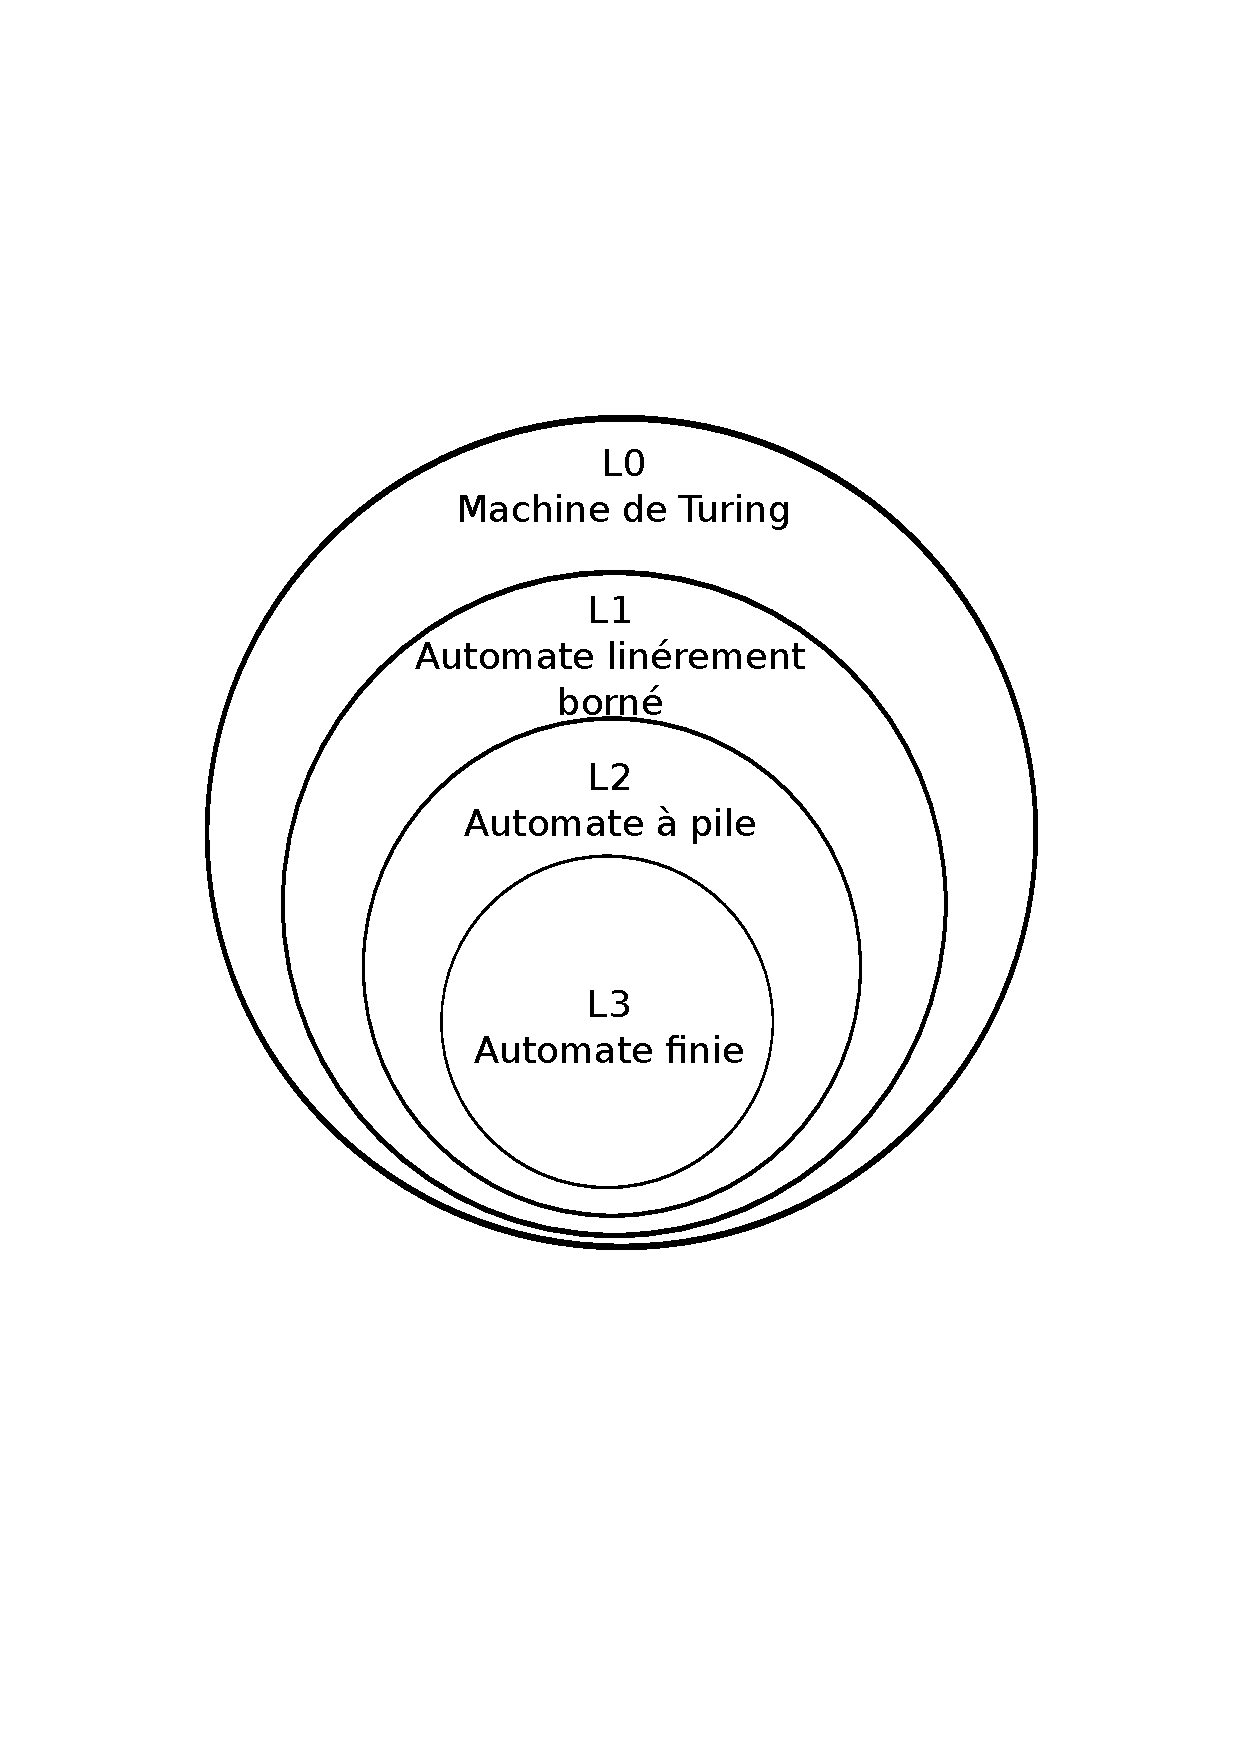
\includegraphics[width=16cm]{part_3/images/hierarchie_chomsky.pdf}
\caption{Hiérarchie de Chomsky}
\end{figure}


\paragraph{Définition} % (fold)
\label{subp:d_finition}

Un langage est de type k, avec $k \in (0,1,2,3)$, s'il existe une grammaire de type k qui l'engendre.
\begin{itemize}
	\item Un langage est régulier s'il est de type 3.
	\item Un langage est algébrique s'il est de type 2.
	\item Un langage est contextuelle s'il est de type 1.
	\item Un langage est récursivement énumérable s'il est de type 0.
\end{itemize}

% paragraph d_finition (end)


\paragraph{Notations} % (fold)
\label{par:notations}

La notation BNF, ou Backus-Naur Forme, est une description d'un langage de programmation. Les terminaux sont les symboles du langages et les non terminaux sont les noms des choses que l'on définit. Les non terminaux sont écrit entre $<>$.

% paragraph notations (end)


\paragraph{Exemple} % (fold)
\label{par:exemple}

Le mot clé $if$ du langage $C++$ a l'une des règles suivantes :\\
$<structure\_if> ::= if\ "(" <conditions> ")"\ "\{" <code> "\}"\ [\ else\ "\{" <code> "\{"\ ]$

% paragraph exemple (end)


% section hi_rarchie_de_chomsky (end)


\section{Grammaires algébriques} % (fold)
\label{sec:grammaires_alg_briques}


\paragraph{Définition} % (fold)
\label{par:d_finition}

Soit une grammaire algébrique $G=(\Sigma, N, P, S)$, une dérivation gauche, respectivement droite, est une dérivation dans laquelle le non terminal dérivé est toujours le plus à gauche, respectivement à droite.

% paragraph d_finition (end)


\paragraph{Définition} % (fold)
\label{par:d_finition}

Un arbre de dérivation est un arbre étiqueté par $\Sigma \cup N \cup \{\epsilon\}$ qui vérifie :

\begin{itemize}
	\item Tout nœud interne, ainsi que la racine, est étiqueté par un non terminal, soit un élément de N.
	\item Si A est l'étiquette d'un nœud $\alpha_1, \alpha_2, ..., \alpha_n$ sont les étiquettes de ses n fils, dans cette arbre, alors $A \rightarrow \alpha_1\alpha_2...\alpha_n \in P$.
\end{itemize}

À tous arbres de dérivations, on peut associer un mot sur $(\Sigma \cup N)^*$ formé des étiquettes des feuilles de l'arbre dans l'ordre dans lequel elles sont visités par un parcours infixe de l'arbre.

% paragraph d_finition (end)


\paragraph{Exemple} % (fold)
\label{par:exemple}

Soit une grammaire algébrique $G=(\{a,b\} , \{S\} , \{S\rightarrow aSbS \mid bSaS \mid \epsilon\} , S)$, on a l'arbre de dérivation suivant :

\begin{center}
	
	\begin{tikzpicture}[level distance=11mm,sibling distance=20mm]
	
	\node {S}
		child{node{a}}
		child{node{S}
			child{node{$\epsilon$}}}
		child{node{b}}
		child{node{S}
			child{node{b}}
			child{node{S}
				child{node{$\epsilon$}}}
			child{node{a}}
			child{node{S}
				child{node{$\epsilon$}}}
			};
	\end{tikzpicture}

\end{center}

On peut avoir plusieurs dérivations pour un mot donné :
\begin{itemize}
	\item $S \Rightarrow aSbS \Rightarrow abS \Rightarrow abbSaS \Rightarrow abbaS \Rightarrow abba$ (Dérivation gauche)
	\item $S \Rightarrow aSbS \Rightarrow aSbbSaS \Rightarrow aSbbaS \Rightarrow abbaS \Rightarrow abba$.
\end{itemize}

% paragraph exemple (end)


\paragraph{Proposition} % (fold)
\label{par:proposition}

Soit une grammaire algébrique $G=(\Sigma,N,P,S)$, avec $A \in N$, alors $A\Rightarrow^* \alpha$ si et seulement s'il existe un arbre de dérivation de racine étiqueté par A et dont le mot associé est $\alpha$.

% paragraph proposition (end)

Le langage engendré par G est l'ensemble des mots sur $\Sigma^*$ associés à des arbres de dérivations de racine étiquette par S (les feuilles sont étiquetées par $\Sigma \cup \{\epsilon\}$).

% section grammaires_alg_briques (end)


\paragraph{Définition} % (fold)
\label{par:d_finition}

La grammaire algébrique G est ambiguë s'il existe $w \in \mathcal{L}(G)$ associés à 2 arbres de dérivations différents partant de l'axiome. Un langage algébrique est ambiguë si toute grammaire qu'il engendre est ambiguë.

% paragraph d_finition (end)


\paragraph{Exemples} % (fold)
\label{par:exemples}

\begin{itemize}
	\item Soit le code suivant :\\
$if(a)\\
if(b)\\
c;\\
else\\
d;$\\

Comment peut-on interpréter ce code avec les 2 règles suivantes :

\begin{itemize}
	\item $if\ (cond)\ instructions ;\ else\ instructions;$
	\item $if\ (cond)\ instructions ;$
\end{itemize}

On obtient alors 2 arbres de dérivations :

\begin{center}
	
	\begin{tikzpicture}[level distance=11mm,sibling distance=20mm]

	\node {}
		child{node{if}}
		child{node{(}}
		child{node{a}}
		child{node{)}}
			child{node{}
				child{node{if}}
				child{node{b}}
				child{node{c}}
				child{node{else}}
				child{node{d}}
			}
		;

	\end{tikzpicture}

\end{center}


\begin{center}
	
	\begin{tikzpicture}[level distance=11mm,sibling distance=20mm]

	\node {}
		child{node{if}}
		child{node{a}}
		child{node{}
			child{node{if}}
			child{node{b}}
			}
		child{node{else}}
		child{node{d}}
	;
	\end{tikzpicture}

\end{center}


\item Soit la grammaire suivante, $G=(\{a,+,*\} , \{S\} , \{S\rightarrow S+S \mid S*S \mid a\} , S)$, pour le mot suivant $a+a*a$ on obtient les arbres suivants :

\begin{center}
	
	\begin{tikzpicture}[level distance=11mm,sibling distance=20mm]

	\node {S}
		child{node{S}
			child{node{a}}
			}
		child{node{+}}
		child{node{S}
			child{node{S}
				child{node{S}
					child{node{a}}
					}
				child{node{*}}
				child{node{S}
					child{node{a}}
					}
				}
			}
		;
		
	\end{tikzpicture}

\end{center}


\begin{center}

	\begin{tikzpicture}[level distance=11mm,sibling distance=20mm]

	\node {S}
		child{node{S}
			child{node{S}
				child{node{a}}
				}
			child{node{+}}
			child{node{S}
				child{node{a}}
				}
			}
		child{node{*}}
		child{node{S}
			child{node{a}}
			}
		;
		
	\end{tikzpicture}
	
\end{center}


\end{itemize}


% paragraph exemples (end)


% chapter grammaires (end)

\chapter{Langage relationnel} % (fold)
\label{cha:langage_relationnel}


\section{Définitions} % (fold)
\label{sec:d_finitions}


\paragraph{Définition} % (fold)
\label{par:d_finition}

L'ensemble des langages rationnels $Rat(\Sigma)$ sur l'alphabet $\Sigma$ est le plus petit ensemble des langages satisfaisant les conditions :

\begin{itemize}
	\item $\varnothing$ est un langage rationnel.
	\item $\{\epsilon\}$ est un langage rationnel.
	\item $\forall a \in \Sigma$, a est un langage rationnel.
	\item Si $\mathcal{L}_1,\mathcal{L}_2 \in Rat(\Sigma)$ alors $\mathcal{L}_1 \cup \mathcal{L}_2 \in Rat(\Sigma)$.
	\item Si $\mathcal{L}_1,\mathcal{L}_2 \in Rat(\Sigma)$ alors $\mathcal{L}_1 . \mathcal{L}_2 \in Rat(\Sigma)$.
	\item Si $\mathcal{L} \in Rat(\Sigma)$ alors $\mathcal{L}^* \in Rat(\Sigma)$.
\end{itemize}

% paragraph d_finition (end)

$Rat(\Sigma)$ est le plus petit ensemble qui contient les langages finis, fermé par Union, Concaténation et Étoile de langages finis, s'appelle une décomposition de Kleene.

% section d_finitions (end)


\section{Expression régulière} % (fold)
\label{sec:expression_r_guli_re}

Les expressions régulières sont une manière plus simple d'écrire une décomposition de Kleene.


\paragraph{Définition} % (fold)
\label{par:d_finition}

Une expression régulière (ou expression rationnelle) pour un alphabet $\Sigma$ est une expression formé par les règles suivantes :

\begin{itemize}
	\item $\varnothing$ est une expression régulière.
	\item $\epsilon$ est une expression régulière.
	\item Si $a \in \Sigma$ alors $a$ est une expression régulière.
	\item Si $\alpha$ et $\beta$ sont des expressions régulières alors $\alpha + \beta$ est une expression régulière.
	\item Si $\alpha$ et $\beta$ sont des expressions régulières alors $\alpha . \beta$ est une expression régulière.
	\item Si $\alpha$ est une expression régulière alors $\alpha^*$ est une expression régulière.
\end{itemize}

% paragraph d_finition (end)


\paragraph{Définition} % (fold)
\label{par:d_finition}

On appelle valeur d'une expression régulière $\alpha$, notée $\mathcal{L}(\alpha)$ le langage désigné par l'expression régulière $\alpha$ définit par :

\begin{itemize}
	\item $\mathcal{L}(\varnothing)=\varnothing$.
	\item $\mathcal{L}(\epsilon)=\{\epsilon\}$.
	\item Si $a \in \Sigma, \mathcal{L}(a)=\{a\}$.
	\item Si $\alpha$ et $\beta$ sont des expressions régulières alors $\mathcal{L}(\alpha + \beta)=\mathcal{L}(\alpha) \cup \mathcal{L}(\beta)$.
	\item Si $\alpha$ et $\beta$ sont des expressions régulières alors $\mathcal{L}(\alpha * \beta)=\mathcal{L}(\alpha) . \mathcal{L}(\beta)$.
	\item Si $\alpha$ est une expression régulière alors $\mathcal{L}(\alpha^*)=(\mathcal{L}(\alpha))^*$.
\end{itemize}

% paragraph d_finition (end)


\paragraph{Exemples} % (fold)
\label{par:exemples}

\begin{itemize}
	\item $\mathcal{L}((ab + \epsilon)bb)=\{abbb , bb\}$.
	\item $\mathcal{L}((a + b)^*bb)$ sont tous les mots de l'alphabet $\Sigma$ se terminant par bb.
\end{itemize}

% paragraph exemples (end)


\paragraph{Attention} % (fold)
\label{par:attention}

$a$ peut désigner 3 choses différentes :
\begin{itemize}
	\item Le symbole $a$ de $\Sigma$.
	\item Le mot $a$ (une suite finie de un symbole).
	\item $a$ est maintenant une expression régulière (dont la valeur est un langage, soit un ensemble de mots $\mathcal{L}(a)=\{a\}$).
\end{itemize}
Il est donc important de préciser de quoi l'on parle au vue des notations.

% paragraph attention (end)


\paragraph{Proposition} % (fold)
\label{par:proposition}

Un langage est rationnelle si et seulement s'il est la valeur d'une expression régulière.

% paragraph proposition (end)


\paragraph{Preuve} % (fold)
\label{par:preuve}

Par isomorphisme (équivalences) des définitions inductives (on part du cas de base pour aller vers des cas généraux).\\

% paragraph preuve (end)

On autorise d'autres notations.

\begin{itemize}
	\item Si $\alpha$ est une expression régulière et $i \in \mathbb{N}$ alors $\alpha^i$ est une expression régulière, $\mathcal{L}(\alpha^i)=((\mathcal{L}(\alpha))^i$.\\
	Exemple : $\alpha=\alpha^3$.
	\item Si $\alpha$ est une expression régulière alors $\alpha^+$ est une expression régulière, $\mathcal{L}(\alpha^+)=(\mathcal{L}(\alpha))^+.$\\
	Exemple : $\alpha\alpha^*=\alpha^+$.
\end{itemize}


\paragraph{Définition} % (fold)
\label{par:d_finition}

2 expressions régulières $\alpha, \beta$ sont équivalentes, noté $\alpha = \beta$ si $\mathcal{L}(\alpha)=\mathcal{L}(\beta)$.

% paragraph d_finition (end)


\paragraph{Exemple} % (fold)
\label{par:exemple}

$(ab + \epsilon)bb=ab^3+b^2$.

% paragraph exemple (end)


Quelques égalités remarquables :

\begin{itemize}
	\item $\alpha + \beta = \beta + \alpha$.
	\item $\alpha + \alpha = \alpha$.
	\item $\alpha + \varnothing = \alpha$.
	\item $\alpha + (\beta + \gamma) = (\alpha + \beta) + \gamma$.
	\item $\alpha . \epsilon = \alpha$.
	\item $\alpha . \varnothing = \varnothing$.
	\item $\alpha . (\beta . \gamma) = (\alpha . \beta) . \gamma$.
	\item $\alpha . (\beta + \gamma) = \alpha . \beta + \alpha . \gamma$.
	\item $\alpha^* = \alpha^* . \alpha^* = ((\alpha^*)^*) = (\epsilon + \alpha)^* = \epsilon + \alpha^+$.
	\item $\varnothing^* = \epsilon^* = \epsilon$.
	\item $(\alpha + \beta)^* = (\alpha^* + \beta^*)^* = (\alpha^* . \beta^*)^* = \alpha^*(\beta . \alpha^*)^* = (\alpha^* . \beta)^* . \alpha^*$.
	\item $\alpha(\beta.\alpha)^* = (\alpha\beta)^*\alpha$.
\end{itemize}


Dans la suite du cours, on identifie $\alpha$ par $\mathcal{L}(\alpha)$.\\
$\alpha \subseteq \beta$ si $\mathcal{L}(\alpha) \subseteq \mathcal{L}(\beta)$. Grâce à la relation d'ordre, on peut obtenir les relations suivantes :


\begin{itemize}
	\item $\alpha \subseteq \beta$ et $\beta \subseteq \alpha$ implique $\alpha = \beta$.
	\item $\alpha \subseteq \alpha$.
	\item Si $\alpha \subseteq \beta$ alors, $\forall \gamma, \gamma\alpha \subseteq \gamma\beta$.
\end{itemize}


$\alpha = \beta$ si $\mathcal{L}(\alpha)=\mathcal{L}(\beta)$. Grâce à la relation d'équivalence, on peut obtenir les relations suivantes :


\begin{itemize}
	\item $\alpha = \alpha$.
	\item $\alpha = \beta$ implique $\beta = \alpha$.
	\item $\alpha = \beta$ et $\beta = \gamma$ implique $\alpha = \gamma$.
\end{itemize}


Si $L$ est le langage rationnel alors $L$ est une expression régulière, $\mathcal{L}(L)=L$.


\paragraph{Théorème} % (fold)
\label{par:th_or_me}

Soit $\alpha$ et $\beta$ 2 expressions régulières, ou langages relationnels, on considère l'équation d'inconnue $X$, $X = \alpha X + \beta$ ($X$ est un langage).


\begin{itemize}
	\item $\alpha^* \beta$ est solution de l'équation.
	\item $\alpha^* \beta$ est la plus petite solution.
	\item Si $\epsilon \not \in \alpha$ alors $\alpha^* \beta$ est l'unique solution.
\end{itemize}

% paragraph th_or_me (end)


\paragraph{Preuve} % (fold)
\label{par:preuve}

\begin{itemize}
	\item $\alpha^* \beta$ est solution de l'équation.\\

	On remplace $X$ par $\alpha^* \beta$ dans $\alpha X + \beta$.\\
	$\alpha X + \beta = \alpha(\alpha^* \beta) + \beta = \alpha^+ \beta + \beta = (\alpha^+ + \epsilon)\beta = \alpha^* \beta=X$.\\
	
	\item $\alpha^* \beta$ est la plus petite solution.\\
	Soit $X$ une solution, on veut montrer $\alpha^* \beta \subseteq X$.\\
	$\alpha^* \beta = (\sum\limits_{i \in \mathbb{N}} \alpha^i)\beta = \sum\limits_{i \in \mathbb{N}}(\alpha^i \beta)$.\\
	On montre par récurrence sur $i$ que $\forall i \in \mathbb{N}, \alpha^i\beta \subseteq X$ :
	
	\begin{itemize}
		\item Pour $i=0, \alpha^i \beta = \alpha^0 \beta = \epsilon \beta = \beta, \beta \subseteq \alpha X + \beta = X$.
		\item Pour $i+1$, on suppose que $\alpha^i \beta \subseteq X$.\\
		$\alpha^{i+1} \beta = \alpha \alpha^i \beta$ donc $\alpha^{i+1} \beta \subseteq \alpha X \subseteq \alpha X + \beta = X$.\\
	\end{itemize}
	
	$\forall \in \mathbb{N}, \alpha^i \beta \subseteq X$. Donc $\alpha^* \beta \subseteq X$, $\alpha^* \beta$ est la plus petite solution.\\

	\item Si $\epsilon \not \in \alpha$ alors $\alpha^* \beta$ est l'unique solution.\\

	Soit $X$ une solution, on va montrer $X \subseteq \alpha^* \beta$.\\
	$X = \alpha X + \beta$\\
	$X = \alpha(\alpha X + \beta)+\beta = \alpha^2 X + \alpha \beta + \beta$\\
	$X = \alpha^2(\alpha X + \beta) + \alpha \beta + \beta = \alpha^3 X + \alpha^2 \beta + \alpha^1 \beta + \alpha^0 \beta$\\
	$X = \alpha^{k+1} X + \alpha^k \beta + ... + \alpha^1 \beta + \alpha^0 \beta = \alpha^{k+1} X + (\alpha^k + ... + \alpha^1 + \alpha^0) \beta$.\\

	Soit $m \in X (m \in \mathcal{L}(X))$, soit $k = \left|m\right|$. Comme $\epsilon \not \in \alpha$, tous les mots de $\alpha^{k+1}$ sont de longueur supérieur ou égale à $k+1$, et donc tous les mots de $\alpha^{k+1} X $ sont de longueur supérieur ou égale à $k+1$. Donc $m \not \in \alpha^{k+1} X$. Donc $m \in (\alpha^k + ... + \alpha^1 + \alpha^0)\beta \in \alpha^* \beta$. Donc $X \subseteq \alpha^* \beta$.\\
\end{itemize}

% paragraph preuve (end)


\paragraph{Théorème} % (fold)
\label{par:th_or_me}

La règle d'Arden, ou Lemme d'Arden, est la règle suivante : Soit $\alpha$ et $\beta$ 2 expressions régulières, ou langages relationnels, on considère l'équation d'inconnue $X$, $X = \alpha X + \beta$ ($X$ est un langage). Si $\epsilon \not \in \alpha$ alors $\alpha^* \beta$ est l'unique solution. Comme $\alpha$ et $\beta$ sont rationnelles, alors $\alpha^* \beta$ est rationnel.

% paragraph th_or_me (end)

Si $\epsilon \in \alpha$ alors la solution n'est pas unique.$\forall \gamma$, tel que $\beta \subseteq \gamma$, alors $\alpha^* \gamma$ est aussi une solution.


\paragraph{Preuve} % (fold)
\label{par:preuve}

$\alpha X + \beta = \alpha (\alpha^* \gamma) + \beta = \alpha^+ \gamma + \beta$\\
$\alpha X + \beta = \alpha^* \gamma + \beta$ (car $\epsilon \in \alpha$) $ = \alpha^* \gamma$ (car $\beta \subseteq \gamma$ dont $\beta \subseteq \alpha^* \gamma$) $= \alpha$.

% paragraph preuve (end)


\paragraph{Analogie avec l'algèbre} % (fold)
\label{par:analogie_avec_l_alg_bre}

Si $\epsilon \not \in \alpha$ alors $\alpha^* \beta$ est une unique solution.\\
$X = \alpha X + \beta \Leftrightarrow X - \alpha X = \beta \Leftrightarrow (1-\alpha) X = \beta \Leftrightarrow X = \frac{\beta}{1-\alpha}$.\\
On suppose que $\alpha \not = 1$, alors $X = (1 + \alpha + \alpha^2 + ... + \alpha^k + ... )\beta$ grâce aux développement limité de $\frac{1}{1-\alpha}$, quand $\alpha \rightarrow 0$.\\
$X = (1 + \alpha + \alpha^2 + ... + \alpha^k + ... )\beta \Leftrightarrow X = \alpha^* \beta$.

% paragraph analogie_avec_l_alg_bre (end)


\paragraph{Remarques} % (fold)
\label{par:remarques}

\begin{itemize}
	\item $X = \epsilon X + \beta \Leftrightarrow \beta \subseteq X$.
	\item $X = \varnothing X + \beta \Leftrightarrow X = \beta$.
\end{itemize}

% paragraph remarques (end)

On considère maintenant le système de n équations à n inconnues $X_1, X_2, ..., X_n$ :

\[
   \left \{
   \begin{array}{cccc}
  		X_{1} = L_{1,1} X_1 + L_{1,2} X_2 + ... + L_{1,n} X_n + L_1\\
    	X_{2} = L_{2,1} X_1 + L_{2,2} X_2 + ... + L_{2,n} X_n + L_2\\
		\vdots\\
    	X_{n} = L_{n,1} X_1 + L_{n,2} X_2 + ... + L_{n,n} X_n + L_n\\
   \end{array}
   \right .
\]

Où les $L_{i,j}$ et $L_i$ sont des langages rationnelles.

\paragraph{Définition} % (fold)
\label{par:d_finition}

Le système ci-dessus est régulier si $\forall i,j, \epsilon \not \in \mathcal{L}_(i,j)$.

% paragraph d_finition (end)


\paragraph{Théorème} % (fold)
\label{par:th_or_me}

Un système d'équations réguliers à n équations et n inconnues à une unique solution qui est un langage rationnel pour chaque inconnue.

% paragraph th_or_me (end)


\paragraph{Preuve} % (fold)
\label{par:preuve}

On peut résoudre le système par une méthode de pivot de Gauss, et on remarque qu'à chaque étape, le système régulier de la forme : $X_1 = (L_{1,1})^*\ (L_{1,2} X_2 + ... + L_{1,n} X_n + L_1)$. On remplace $X_1$ dans toutes les équations et l'on recommence ainsi pour chaque une des inconnues.

% paragraph preuve (end)


\paragraph{Exemple} % (fold)
\label{par:exemple}

Soit le système suivant, avec $a,b \not \in \epsilon$ :\\
\[
   \left \{
   \begin{array}{cc}
  		X = aX + vY + \epsilon\\
    	Y = bX + aY\\
   \end{array}
   \right .
\]

\[
   \left \{
   \begin{array}{cc}
  		X = aX + b(a^*bX) + \epsilon\\
    	Y = a^*bX\\
   \end{array}
   \right .
\]

\[
   \left \{
   \begin{array}{cc}
  		X = (a+ba^*b)X + \epsilon\\
    	Y = a^*bX\\
   \end{array}
   \right .
\]

\[
   \left \{
   \begin{array}{cc}
  		X = (a+ba^*b)^*\\
    	Y = a^*b(a+ba^*b)^*\\
   \end{array}
   \right .
\]

% paragraph exemple (end)

% section expression_r_guli_re (end)


\section{Grammaires régulières} % (fold)
\label{sec:grammaires_r_guli_res}

Toutes les règles de production de la forme $A \rightarrow w$ ou $A \rightarrow wB$ avec $A$ et $B$ des non terminaux et $w$ un mot sur l'alphabet terminal. Un langage est régulier s'il est engendré par une grammaire régulière.


\paragraph{Proposition} % (fold)
\label{par:proposition}

Tout langage fini est régulier.

% paragraph proposition (end)


\paragraph{Preuve} % (fold)
\label{par:preuve}

Soit $L = \{w_1, w_2, ... , w_n\}$, $L$ est engendré par une grammaire $G = (\Sigma , \{S\}, \{S \rightarrow w, S \rightarrow w_1 \mid w_2 \mid ... \mid w_n\},S)$.
Une grammaire linéaire gauche a des règles de productions de la forme, $A \rightarrow w$ ou $A \rightarrow Bw$. On a une équivalence avec les grammaires régulières est le terme du langage engendré.

% paragraph preuve (end)


\paragraph{Proposition} % (fold)
\label{par:proposition}

Tout langage régulier est engendré par une grammaire $G=(\Sigma,N,P,S)$, dont les règles de productions sont toutes de la forme $A \rightarrow aB$ (avec $A,B \in N$, des non terminaux et $a \in \Sigma$, un terminal) ou $A \rightarrow \epsilon$, avec $A \in N$.

% paragraph proposition (end)


\paragraph{Preuve} % (fold)
\label{par:preuve}

Soit la grammaire régulière $G=(\Sigma,N,P,S)$. Soit une règle de $P$ qui n'a pas la bonne forme.

\begin{itemize}
	\item $A \rightarrow a_1a_2 ... a_k B$ avec $k \geq 2$.\\
	On ajoute k-1 non terminaux $B_1, B_2, ..., B_{k-1}$ à $N$, et on remplace la règle par k règles, on obtient : \\
	$A \rightarrow a_1 B_1$\\
	$B_1 \rightarrow a_2 B_2$\\
	$\vdots$\\
	$B_{k-1} \rightarrow a_k B$

	\item $A \rightarrow a_1a_2 ... a_k$ avec $k \geq 1$. On ajoute k non terminaux $B_1 B_2 ... B_k$ à $N$ et on remplace par les $k+1$ règles, on obtient :\\
	$A \rightarrow a_1 B_1$\\
	$B_1 \rightarrow a_2 B_2$\\
	$\vdots$\\
	$B_{k-1} \rightarrow a_k B_k$\\
	$B_k \rightarrow \epsilon$

	\item $A \rightarrow B$, avec $k=0$.
	\begin{itemize}
		\item Si $A = B$, alors on a la règle $A \rightarrow A$ que l'on peut supprimer.
		\item Si $A \not = B$. Soit $B \rightarrow \alpha_1 \mid \alpha_2 \mid ... \mid \alpha_n$, toutes les règles avec $B$ à gauche. On remplace $A \rightarrow B$ par $A \rightarrow \alpha_1 \mid \alpha_2 \mid ... \mid \alpha_n$.
	\end{itemize}

\end{itemize}

% paragraph preuve (end)


\paragraph{Remarque} % (fold)
\label{par:remarque}

Pour une grammaire régulière, on obtient l'arbre de dérivation suivant :

\begin{center}
	\begin{tikzpicture}[level distance=11mm,sibling distance=20mm]
	
	\node{S}
		child{node{$a_{1,1}$}}
		child{node{$a_{1,2}$}}
		child{node{...}}
		child{node{$a_{1,n}$}}
		child{node{$A_1$}
			child{node{$a_{2,1}$}}
			child{node{$a_{2,2}$}}
			child{node{...}}
			child{node{$A_2$}
				child{node{...}
					child{node{$A_k$}
						child{node{$a_{k,1}$}}
						child{node{$a_{k,2}$}}
						child{node{...}}
						child{node{$a_{k,n_k}$}}
						}
					}
				}
			}
		;

	\end{tikzpicture}
\end{center}

% paragraph remarque (end)


\paragraph{Remarques} % (fold)
\label{par:remarques}

Pour un arbre de dérivation il y a une seule dérivation qui lui correspond, c'est-à-dire que la dérivation gauche est équivalente à la dérivation droite.\\

% paragraph remarques (end)

Soit la grammaire $G=(\Sigma,N,P,S)$, soit $A \in N$, on peut définir $\mathcal{L}(A)=\{ w \in \Sigma^* \mid A \Rightarrow^* w \}$


\paragraph{Proposition} % (fold)
\label{par:proposition}

Soit $G=(\Sigma,N,P,S)$ une grammaire régulière alors $\forall A \in N, \mathcal{L}(A)$ est un langage régulière.

% paragraph proposition (end)


\paragraph{Preuve} % (fold)
\label{par:preuve}

$\mathcal{L}(A)$ est le langage engendré par $(\Sigma,N,P,A)$ avec $\Sigma,N,P$ les même que G.

% paragraph preuve (end)


% section grammaires_r_guli_res (end)


\section{Automate d'états fini} % (fold)
\label{sec:automate_d_tats_fini}

\paragraph{Définition} % (fold)
\label{par:d_finition}

Un automate d'états fini, ou automate fini, c'est un quintuplet $(\Sigma,Q,\Delta,D,F)$ avec:

\begin{itemize}
	\item $\Sigma$ est un alphabet, un ensemble fini de symboles.
	\item $Q$ est un ensemble fini d'états.
	\item $\Delta$ est un ensemble de relations, $\Delta \subseteq Q \times \Sigma \times Q$. Un élément $(q,x,q')$ de $\Delta$ est appelé une transition. On passe de l'état $q$ à l'état $q'$ en acceptant $x$.
	\item $D$ est l'ensemble des états initiaux, $D \subseteq Q$.
	\item $F$ est l'ensemble des états finaux, $F \subseteq Q$.
\end{itemize}

% paragraph d_finition (end)


\paragraph{Diagramme de transition} % (fold)
\label{par:diagramme_de_transition}

L'automate est vu comme un graphe orienté et étiqueté. On prendra par la suite les notations suivantes :

\begin{itemize}
	\item Un état $q \in Q$\\

	\begin{tikzpicture}
	  \tikzstyle{every state}=[draw=black,text=black]
	
	  \node[state] (Q)                    {$q$};
	
	\end{tikzpicture}\\

	\item Un état initial $q_0 \in D$\\

	\begin{tikzpicture}
	\tikzstyle{every state}=[draw=black,text=black]
	
		\node[initial,state]	(Q)	{$q_0$};
	
	\end{tikzpicture}\\

	\item Un état final $q_k \in F$\\

	\begin{tikzpicture}
	\tikzstyle{every state}=[draw=black,text=black]
	
		\node[state,accepting]	(Q)	{$q_k$};
	
	\end{tikzpicture}\\

	ou\\

	\begin{tikzpicture}[shorten >=1pt,node distance=2cm,>=stealth',thick]
	\tikzstyle{every state}=[draw=black,text=black]

		\node[state]	(Q)	{$q_k$};
		\coordinate[right of=Q] (dQ);
		\draw[->]	(Q)	to[bend right]	node[auto]	{}	(dQ);
	\end{tikzpicture}\\

	\item Une transition $(q,x,q') \in \Delta$\\

	\begin{tikzpicture}[->,>=stealth',shorten >=1pt,auto,node distance=2.8cm]
	\tikzstyle{every state}=[draw=black,text=black]
	
		\node[state]	(1)						{$q_1$};
		\node[state]	(2)	[right of=1]		{$q_2$};

	\path	(1)	edge	node{$x$}	(2);
	
	\end{tikzpicture}\\

\end{itemize}

% paragraph diagramme_de_transition (end)


\paragraph{Exemple} % (fold)
\label{par:exemple}

Soit l'automate défini de la manière suivante $(\{a,b\},\{1,2\},\{(1,a,1),(1,b,2),(2,a,1)\},\{1\},\{1\})$\\

\begin{tikzpicture}[->,>=stealth',shorten >=1pt,auto,node distance=2.8cm]
\tikzstyle{every state}=[draw=black,text=black]
	
	\node[state,initial,accepting]					(1)	{$1$};
	\node[state]					[right of=1]	(2)	{$2$};

	\path	(1)	edge	[loop above]	node{$a$}	(1)
				edge 	[bend left]		node{$b$}	(2)
			(2)	edge 	[bend left]		node{$a$}	(1);
			% (2)	edge					node($a$)	(1);

\end{tikzpicture}

% paragraph exemple (end)


\paragraph{Définition} % (fold)
\label{par:d_finition}

Soit l'automate $A=(\Sigma,Q,\Delta,D,F)$, soit $w$ un mot sur $\Sigma$ de longueur $k$ ($\left|w\right|=k$) et pour tout $i \leq k$, soit $x_i \in \Sigma$ tel que $w=x_1 x_2 \ldots x_k$.\\
Le mot est accepté, ou reconnu, par l'automate $A$, s'il existe une suite d'état $q_0, q_1, \ldots, q_k$ tel que:

\begin{itemize}
	\item $q_0 \in D$, l'état initial.
	\item $\forall i, 1 \leq i \leq k$, on a une transition de la forme $(q_{i-1},x,q_{i}) \in \Delta$.
	\item $q_k \in F$, l'état final.
\end{itemize}

% paragraph d_finition (end)


\paragraph{Exemple} % (fold)
\label{par:exemple}

Soit l'automate $A=(\{a,b\},\{1,2\},\{(1,a,1),(1,b,2),(2,a,1)\},\{1\},\{1\})$
\begin{itemize}
	\item $w=abaa$ est un mot accepté par l'automate.
	\item $w=abaab$ n'est pas un mot par l'automate.
\end{itemize}

% paragraph exemple (end)


\paragraph{Définition} % (fold)
\label{par:d_finition}

Soit $A=(\Sigma,Q,\Delta,D,F)$, le langage reconnu, ou accepté, par $A$, noté $\mathcal{L}(A)$ est $\mathcal{L}(A)=\{w \in \Sigma^* \mid w\ est\ reconnu\ par\ A\}$.

% paragraph d_finition (end)


\paragraph{Exemple} % (fold)
\label{par:exemple}

L'ensemble des mots tel que tout $b$ est suivi d'un $a$, est l'expression $(a+ba)^*$.

% paragraph exemple (end)


\paragraph{Définition} % (fold)
\label{par:d_finition}

Deux automates $A$ et $B$ sont équivalents si $\mathcal{L}(A)=\mathcal{L}(B)$.

% paragraph d_finition (end)


\paragraph{Définition} % (fold)
\label{par:d_finition}

Un langage $L \subseteq \Sigma^*$ est reconnaissable s'il existe un automate $A$ tel que $L=\mathcal{L}(A)$.

% paragraph d_finition (end)


\paragraph{Remarque} % (fold)
\label{par:remarque}

$\epsilon \in \mathcal{L}(A) \Leftrightarrow D \cap F \not = \varnothing$.

% paragraph remarque (end)


\paragraph{Définition} % (fold)
\label{par:d_finition}

$\forall q \in Q$, on note $\mathcal{L}(q)$, le langage reconnu par l'automate $A=(\Sigma,Q,\Delta,\{q\},F)$. Les $\mathcal{L}(q)$ sont des langages reconnaissables.

% paragraph d_finition (end)


\paragraph{Proposition} % (fold)
\label{par:proposition}

$\mathcal{L}(A) = \bigcup\limits_{q \in D} \mathcal{L}(q)$.

% paragraph proposition (end)


\paragraph{Preuve} % (fold)
\label{par:preuve}

Trivial par l'ensemble des définitions.

% paragraph preuve (end)


\paragraph{Définition} % (fold)
\label{par:d_finition}

Un automate $A$ est déterministes si :

\begin{itemize}
	\item $\left|D\right| = 1$, un seul état initial.
	\item Pour tout état, pour tout symbole, on a au plus une transition partant de cette état étiqueté par ce symbole. $\forall q \in Q, \forall x \in \Sigma, \left| \{ q' \in Q \mid (q,x,q') \in \Delta \} \right| \leq 1$.
\end{itemize}

C'est-à-dire que $\Delta$ est le graphe d'une fonction éventuellement partielle, de $Q \times \Sigma$ dans $Q$.\\

Un automate $A$ est complet si :

\begin{itemize}
	\item Pour tout état, pour tout symbole, on a au moins une transition partant de cette état étiqueté par ce symbole. $\forall q \in Q, \forall x \in \Sigma, \left| \{ q' \in Q \mid (q,x,q') \in \Delta \} \right| \geq 1$.\\
\end{itemize}

Un automate $A$ est déterministe complet si :

\begin{itemize}
	\item $\left| D \right| = 1$, un seul état initial.
	\item Pour tout état, pour tout symbole, on a une transition partant de cette état étiqueté par ce symbole. $\forall q \in Q, \forall x \in \Sigma, \left| \{ q' \in Q \mid (q,x,q') \in \Delta \} \right| = 1$.\\
\end{itemize}

Dans un automate déterministe complet, pour tout mot $w$, il existe un seul chemin étiqueté par $w$.

% paragraph d_finition (end)


\paragraph{Exemple} % (fold)
\label{par:exemple}

\begin{itemize}
	\item Soit l'automate $A = (\{a,b\} , \{1,2\} , \{(1,a,1) , (1,b,2) , (2,a,1)\} , \{1\} , \{1\})$ est déterministe mais non complet.
	\item Soit l'automate $A = (\{a,b\} , \{1,2\} , \{(1,a,1) , (1,a,2) , (2,b,1)\} , \{1\} , \{1\})$ est non déterministe et non complet.
\end{itemize}

\begin{center}
	\begin{tikzpicture}[->,>=stealth',shorten >=1pt,auto,node distance=2.8cm]
	\tikzstyle{every state}=[draw=black,text=black]
		
		\node[state,initial,accepting]					(1)	{$1$};
		\node[state]					[right of=1]	(2)	{$2$};
	
		\path	(1)	edge	[loop above]	node{$a$}	(1)
					edge 	[bend left]		node{$a$}	(2)
				(2)	edge 	[bend left]		node{$b$}	(1);
				% (2)	edge					node($a$)	(1);
	
	\end{tikzpicture}
\end{center}



% paragraph exemple (end)


\paragraph{Remarque} % (fold)
\label{par:remarque}

La relation de transition $\Delta \subseteq Q \times \Sigma \times Q$ peut être vue comme une fonction, notée $\Delta$, de $Q \times \Sigma \rightarrow \mathcal{P}(Q)$, avec $\mathcal{P}(Q)$ l'ensemble des parties de $Q$ noté aussi $\mathcal{L}^Q$.

% paragraph remarque (end)


\paragraph{Exemple} % (fold)
\label{par:exemple}

Soit l'automate $A = (\{a,b\} , \{1,2\} , \{(1,a,1) , (1,a,2) , (2,b,1)\} , \{1\} , \{1\})$, on a :\\

\begin{itemize}
	\item $\Delta(1,a) = \{1,2\}$.
	\item $\Delta(1,b) = \varnothing$.
	\item $\Delta(2,a) = \varnothing$.
	\item $\Delta(2,b) = \{1\}$.
\end{itemize}

% paragraph exemple (end)


\paragraph{Remarques} % (fold)
\label{par:remarques}

\begin{itemize}
	\item La fonction $\Delta$ peut être représenté par la table suivante :\\

	\begin{center}
		\begin{tabular}{|l|c|r|}
			\hline
			$\Delta$ & $a$ & $b$\\

			\hline
			1 & $\{1,2\}$ & $\varnothing$\\

			\hline
			2 & $\varnothing$ & $\{1\}$\\

			\hline
		\end{tabular}
	\end{center}
	
	\item Cette fonction de transition $\Delta : Q \times \Sigma \rightarrow \mathcal{P}(Q)$ peut être étendue à une fonction, notée $\Delta$ de $Q \times \Sigma^*$ dans $\mathcal{P}(Q)$, de la manière suivante :

	\begin{itemize}
		\item $\forall q \in Q, \Delta(q,\epsilon) = \{q\}$.
		\item $\forall q \in Q, \forall x \in \Sigma, \forall w \in \Sigma^*, \Delta(q,xw) = \bigcup\limits_{q' \in \Delta(q,x)} \Delta(q',w)$.
	\end{itemize}

\end{itemize}

% paragraph remarques (end)


\paragraph{Preuve} % (fold)
\label{par:preuve}

C'est bien une extension car \\$\forall q \in Q, \forall x \in \Sigma, \Delta(q,x) = \bigcup\limits_{q' \in \Delta(q,x)} \Delta(q',\epsilon) = \bigcup\limits_{q' \in \Delta(q,x)} \{q'\} = \Delta(q,x)$.

% paragraph preuve (end)


\paragraph{Exemple} % (fold)
\label{par:exemple}

Soit l'automate $A = (\{a,b\} , \{1,2\} , \{(1,a,1) , (1,a,2) , (2,b,1)\} , \{1\} , \{1\})$, on a :\\

$\Delta(1,aba)=\Delta(1,ba) \cup \Delta(2,ba) =\varnothing \cup \Delta(1,a)=\Delta(1,\epsilon) \cup \Delta(2,\epsilon) = \{1\} \cup \{2\} = \{1,2\}$.\\

% paragraph exemple (end)


\paragraph{Remarque} % (fold)
\label{par:remarque}

La fonction de transition $\Delta : Q \times \Sigma^* \rightarrow \mathcal{P}(Q)$ peut être étendu à une fonction, noté $\Delta$, de $\mathcal{P}(Q) \times \Sigma^*$ dans $\mathcal{P}(Q)$ de la manière suivante :\\

$\forall X \subseteq Q, \forall w \in \Sigma^*, \Delta(X,w) = \bigcup\limits_{q \in X}\Delta(q,w)$.

% paragraph remarque (end)


\paragraph{Proposition} % (fold)
\label{par:proposition}

Un mot $w \in \Sigma^*$ est accepté par $(\Sigma,Q,\Delta,D,F)$ si et seulement si $\Delta(D,w) \cap F \not = \varnothing$.

% paragraph proposition (end)


\paragraph{Preuve} % (fold)
\label{par:preuve}

On fait une récurrence sur la longueur du mot $w$. 

% paragraph preuve (end)


\paragraph{Conséquence} % (fold)
\label{par:cons_quence}

$\mathcal{L}(A) = \{ w \in \Sigma^* \mid \Delta(D,w) \cap F \not = \varnothing\}$.

% paragraph cons_quence (end)


\paragraph{Remarques} % (fold)
\label{par:remarques}

\begin{itemize}
	\item Si $A=(\Sigma,Q,\Delta,D,F)$ est déterministe alors à sa relation de transition correspond une fonction dont toutes les images sont des singletons ou $\varnothing$. A cette fonction, on peut faire correspondre une fonction $\delta : Q \times \Sigma \rightarrow Q$, définie par $\forall q \in Q, \forall x \in \Sigma$, s'il existe $q'$ tel que $(q,x,q') \in \Delta$ alors $q'$ est unique ($\Delta(q,x) = \{q'\}$) et $\delta(q,x)=q'$, s'il n'existe pas $q'$ alors $\delta(q,x)$ n'est pas défini ($\delta$ est une fonction partielle)($\Delta(q,x)=\varnothing$).

	\item Si $A$ est déterministe alors $D=\{q_0\}$, un seul état initial. L'automate $A$ pourra être désigné indifféremment par $(\Sigma,Q,\Delta,D,F)$, par définition de l'automate d'états fini, ou par le quintuplet $(\Sigma,Q,\delta,q_0,F)$, par définition de l'automate d'états finis déterministe.

	\item Si $A$ est déterministe complet alors $\delta$ est une fonction totale\\
	$\forall q \in Q, \forall x \in \Sigma, \delta(q,x)$ est défini.

	\item La fonction $\delta$ peut être étendu à $\delta : Q \times \Sigma^* \rightarrow Q$, si $A$ est complet, cette extension de $\delta$ est totale.
\end{itemize}

% paragraph remarques (end)


\paragraph{Proposition} % (fold)
\label{par:proposition}

Un mot de $w \in \Sigma^*$ est accepté par $A=(\Sigma,Q,\delta,q_0,F)$ déterministe si et seulement si $\delta(q_0,w) \in F$.

% paragraph proposition (end)


\paragraph{Preuve} % (fold)
\label{par:preuve}

Évidant en appliquant les définitions.

% paragraph preuve (end)


\paragraph{Proposition} % (fold)
\label{par:proposition}

Tout automate est équivalent à un automate complet.

% paragraph proposition (end)


\paragraph{Preuve} % (fold)
\label{par:preuve}

Soit $A=(\Sigma,Q,\Delta,D,F)$, un automate quelconque. Si $A$ est non complet :

\begin{itemize}
	\item On ajoute un nouvel état $\Pi$ à $Q$.
	\item $\forall q \in Q, \forall x \in \Sigma$, si $\Delta(q,x)=\varnothing$, alors on ajoute $(q,x,\Pi)$ à $\Delta$.
	\item $\forall x \in \Sigma$, on ajoute $(\Pi,x,\Pi)$ à $\Delta$.
\end{itemize}

L'automate obtenu $(\Sigma , Q \cup \{\Pi\} , \Delta \cup \{ (q,x,\Pi) \mid \Delta(q,x) = \varnothing \} \cup \{ (\Pi,x,\Pi) \mid x \in \Sigma \} , D , F)$ est complet et équivalent à $A$. Tous les nouveaux chemins se retrouvent dans l'état $\Pi$. L'état $\Pi$, qui est ajouté pour compléter l'automate, est puits, ou l'état poubelle.

% paragraph preuve (end)


\paragraph{Proposition} % (fold)
\label{par:proposition}

Tout automate est équivalent à un automate déterministe.

% paragraph proposition (end)


\paragraph{Preuve} % (fold)
\label{par:preuve}

Soit l'automate $A=(\Sigma,Q,\Delta,D,F)$. L'algorithme pour construire un automate déterministe équivalent noté $Det(A)$ est le suivant : \\
$Det(A) = (\Sigma , \mathcal{P}(Q) , \delta , D , \{X \in \mathcal{P}(Q) \mid X \cap F \not = \varnothing\} )$ avec $\delta$ défini par : $\forall X \in \mathcal{P}(Q), \forall x \in \Sigma, \delta(X,x)=\Delta(X,x)=\bigcup\limits_{q \in X} \Delta(q,x)$.

% paragraph preuve (end)


\paragraph{Idée de construction} % (fold)
\label{par:id_e_de_construction}

Partir de $D$. On suit en parallèle tous les chemins possibles dans $A$, donc à chaque instant on se trouve dans un ensemble d'états.

% paragraph id_e_de_construction (end)


\paragraph{Exemple} % (fold)
\label{par:exemple}

Soit l'automate $A = (\{a,b\} , \{1,2\} , \{(1,a,1) , (1,a,2) , (2,b,1)\} , \{1\} , \{1\})$, on peut faire la construction suivante :\\
$Det(A) = (\{a,b\} , \{\varnothing , \{1\} , \{2\} , \{1,2\}\} , \{ (\varnothing,a,\varnothing) , (\varnothing,b,\varnothing) , (\{1\},a,\{1,2\}) , (\{1\},b,\varnothing) ,(\{1,2\},a,\{1,2\}) , \linebreak[4] (\{1,2\},b,\{1\}) , (\{2\},a,\varnothing) , (\{2\},b,\{1\}) \} , \{1\} , \{ \{1\}  , \{1,2\} \} )$


\begin{table}[h!]
\begin{minipage}[t]{.6\linewidth}

	\begin{tikzpicture}[->,>=stealth',shorten >=1pt,auto,node distance=2.8cm]
	\tikzstyle{every state}=[draw=black,text=black]
		
		\node[state,initial,accepting]					(1)	{$1$};
		\node[state]					[right of=1]	(2)	{$2$};
	
		\path	(1)	edge	[loop above]	node{$a$}	(1)
					edge 	[bend left]		node{$a$}	(2)
				(2)	edge 	[bend left]		node{$b$}	(1);
	
	\end{tikzpicture}

\end{minipage}
\begin{minipage}[t]{.6\linewidth}

	\begin{tikzpicture}[->,>=stealth',shorten >=1pt,auto,node distance=2.8cm]
	\tikzstyle{every state}=[draw=black,text=black]
		
		\node[state,initial,accepting]	(A)							{$1$};
		\node[state,accepting]			(B)	[right of=A]		{$1,2$};
		\node[state]					(C)	[above right of=A]		{$\varnothing$};
		% \node[state,initial,accepting]					(1)	{$1$};
		% \node[state]					[right of=1]	(2)	{$2$};
	
		\path	(A)		edge					node{$b$}	(C)
						edge 	[bend left]		node{$a$}	(B)
				(B)		edge	[loop above]	node{$a$}	(B)
						edge 	[bend left]		node{$b$}	(A)
				(C)		edge	[loop right]	node{$a$}	(C)
						edge 	[loop left] 	node{$b$}	(C);
	
	\end{tikzpicture}

\end{minipage}
\end{table}

% paragraph exemple (end)


% section automate_d_tats_fini (end)


% chapter langage_relationnel (end)


\end{document}
